\chapter{GUI-Entwurf}
\label{chapter:gui}

Eine Software kann noch so gut geplant und durchstrukturiert sein, wenn die Benutzeroberfläche jedoch unübersichtlich ist und nicht bedient werden kann, dann ist der gesamte Rest hinfällig. Daher ist es nötig sich bereits im Vorfeld eine mögliche Front-End-Gestaltung zu überlegen. In Anbetracht der Tatsache, dass der Programmentwurf in Java umgesetzt werden wird, haben wir beim GUI-Entwurf auf die Gestaltung von zu umständlichen und modernen Bestandteilen, wie man sie heute auf den meisten Webseiten sehen kann, verzichtet und uns auf die grundlegenden Bestandteile fokussiert. 


Übergeordnet soll in der gesamten Anwendung ein einheitliches Design vorliegen. Darum haben wir uns bereits zu Beginn auf ein Farbschema abgestimmt. Basierend auf einer Mitarbeiterumfrage haben wir uns für ein rötlich-rosa Farbschema entschieden, sodass die Farben (in Hexwerten) \textbf{\#DE639A}, \textbf{\#E388B1}, \textbf{\#D7A6B3}, \textbf{\#F1E2E2}, \textbf{\#707070} ihre Anwendung fanden. 

Der Nutzer soll die Möglichkeit haben das Design der Benutzeroberfläche auf ein 'Dark Theme' umzustellen. Durch die Auswahl des 'Dark Themes' soll die Benutzeroberfläche der Anwendung dunkler dargestellt werden. Dazu haben wir uns zusätzlich für folgendes Farbschema entschieden (siehe Abbildung \ref{mu:darkmode}).

\begin{figure}[!ht]
    \centering
    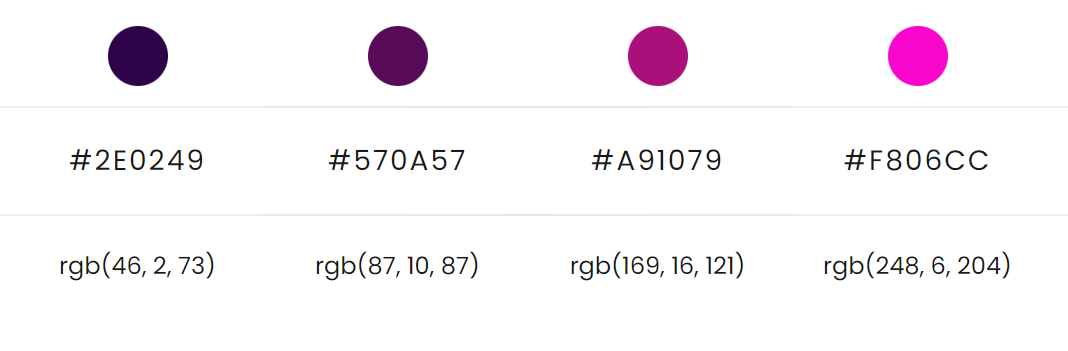
\includegraphics[width=\textwidth]{Bilder/Mockup/colorscheme_darkmode.PNG}
    \caption{Dark Theme Farbschema}
    \label{mu:darkmode}
\end{figure}

\newpage

\section{Diagramm}

\begin{figure}[!ht]
    \centering
    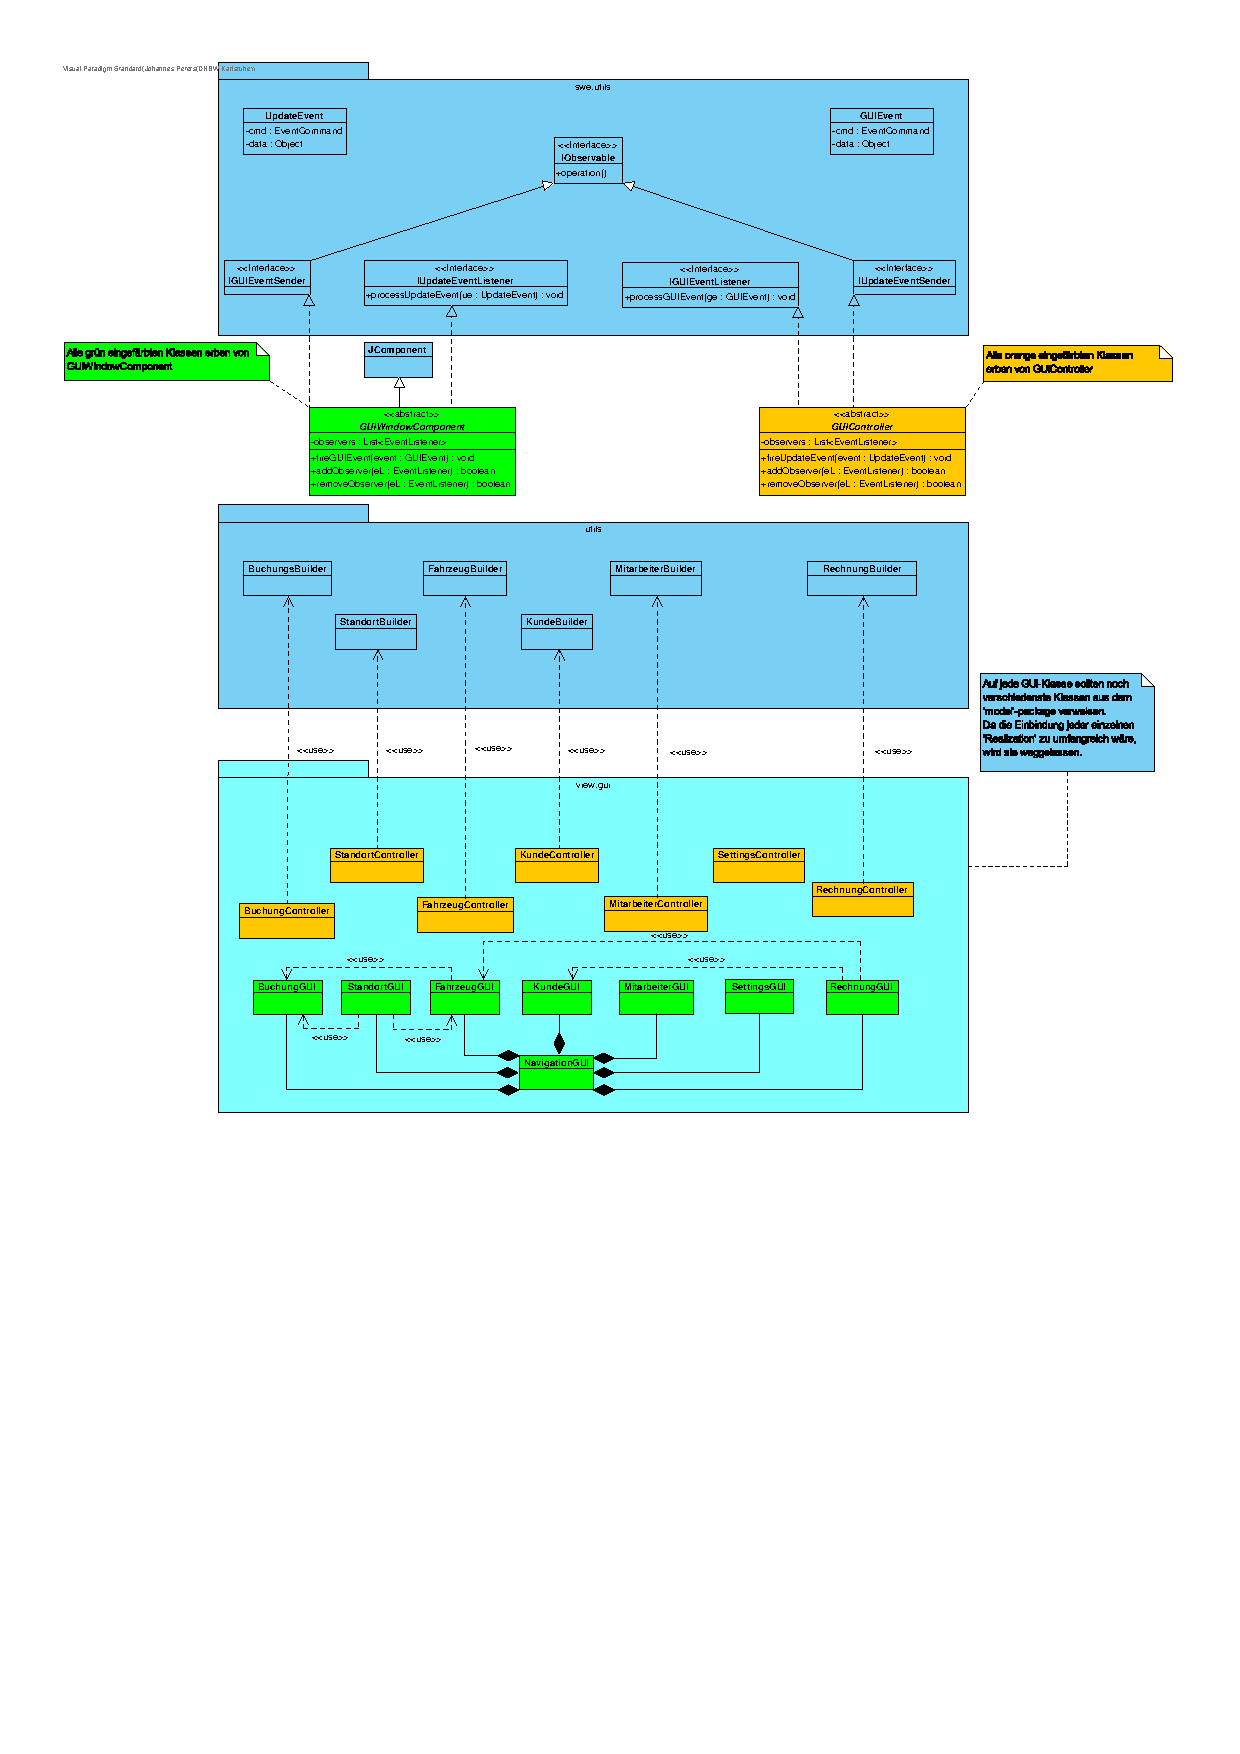
\includegraphics[width=\textwidth, trim = 0cm 10cm 0cm 0cm]{Bilder/Diagramme/EKD_GUI.pdf}
    \caption{Entwurfsklassendiagramm: GUI}
    \label{img:ekd_gui}
\end{figure}

\newpage

\section{Mock-Up}

Der Aufbau der Benutzeroberfläche ist an die Vorgehensweise bei mobilen Android Anwendungen angelehnt und basiert auf dem Konzept von 'Activity' und 'Fragments'. 
Die NavigationGUI dient dabei als 'Activity' und stellt eine Navigationsleiste bereit, die es den Anwendern ermöglicht zwischen verschiedenen Verwaltungsbereichen hin und her zu wechseln. 
Diese Navigationsleiste befindet sich vertikal angeordnet auf der linken Seite des Bildschirms, während der gesamte obere Bereich den Schriftzug des Unternehmens und das Firmenlogo zeigt. 
Die Hauptfläche des Bildschirms erscheint als das 'Fragment', welches je nach Verwaltungsbereich unterschiedlich gestaltet ist. 
Um Rücksicht auf die technisch weniger versierten Mitarbeiter zu nehmen, soll die Aufteilung der Fragment-Fläche bei den unterschiedlichen Bereichen so ähnlich wie möglich sein.
Grundsätzlich besteht daher jede Fragment-Seite aus zwei Feldern.
Das linke Feld zeigt eine Liste, in der sich meist alle Einträge des betroffenen Verwaltungsobjekts befinden, das rechte Feld dient der Detailansicht bei Auswahl eines Datensatzes. 

\subsection{Fahrzeuge verwalten}

Sobald ein Anwender zur Fahrzeugverwaltung navigiert, erhält er eine Übersicht an allen vorhanden Fahrzeugen aus der Datenbasis. 
Diese Datenabfrage wird automatisch beim Aufrufen der GUI ausgeführt. 
Wie auch bei vielen anderen Listenanwendungen gibt es die Möglichkeit nach bestimmten Dateneinträgen zu Suchen oder zu Filtern. 
Das durch den Klick auf den Button oder das Enter in der Texteingabe wird ein GUIEvent erzeugt, welches eine modifizierte Datenabfrage an die Datenbasis absetzt.
Mittel eines UpdateEvents wird die Liste neu geladen und die geänderte Datenauswahl wird in der Liste angezeigt. 
Sofern ein Fahrzeugeintrag ausgewählt wird, soll auf der rechten Bildschirmseite die Detailansicht des Fahrzeuges erscheinen. 
Auch hier wird mittels eines GUIEvents durch das Klicken auf den entsprechenden Listeneintrag auf eine Mauseingabe gewartet, welches die Detailinformationen auf den Bildschirm schreibt. 

\newpage

\begin{figure}[!ht]
    \centering
    \includegraphics[width=\textwidth]{Bilder/Mockup/Web 1920 – 3.png}
    \caption{Mock-Up: Liste an Fahrzeugen}
    \label{mu:fahrzeugliste}
\end{figure}

\begin{figure}[!ht]
    \centering
    \includegraphics[width=\textwidth]{Bilder/Mockup/Web 1920 – 4.png}
    \caption{Mock-Up: Detailansicht eines Fahrzeugs}
    \label{mu:fahrzeugdetails}
\end{figure}

\newpage

\textbf{Fahrzeug löschen}

Exemplarisch für Fahrzeuge, doch übertragbar auch alle anderen Datenobjekte, ist die Manipulationen der Datensätze möglich. 
Zu den Manipulationsmöglichkeiten gehören 'Anlegen', 'Bearbeiten' und 'Löschen'. 
Die Interaktion zum Löschen des ausgewählten Fahrzeug-Datensatzes erfolgt über ein einfaches Pop-Up-Fenster.  
Der Anwender muss diesen Dialog bestätigen, wenn er den Datensatz löschen möchte.
Da die bestehende Datenbasis durch das Löschen bearbeitet wird, erzeugt diese Aktion ein UpdateEvent und entfernt den betroffenen Datensatz aus der Datenbasis.
Nach dem Löschen wird der Anwender auf die Fahrzeug-Startseite zurückverwiesen, jedoch wird in der Liste der gelöschte Eintrag durch das ausgelöste UpdateEvent entfernt. 


\begin{figure}[!ht]
    \centering
    \includegraphics[width=\textwidth]{Bilder/Mockup/Web 1920 – 5.png}
    \caption{Mock-Up: Löschen eines Fahrzeugs}
    \label{mu:loeschen}
\end{figure}

\newpage

\textbf{Fahrzeug bearbeiten}

Das Bearbeiten eines Datensatzes ist so einfach wie möglich gestaltet. 
Der einzige Unterschied von der Bearbeitungs-GUI zur Detail-GUI ist, dass alle Felder, die bearbeitet werden können sollen, entweder zu einem Eingabefeld oder einer Drop-Down-Liste werden. 
Im folgenden Beispiel werden nur die Felder 'Reifen' und 'Ausrüstung' bearbeitbar. 
Da es sehr unwahrscheinlich ist, dass sich bei einem bereits vorhandenen Fahrzeug der Hersteller, das Modell, die Fahrzeugklasse oder das Baujahr ändern, soll es nicht bearbeitbar sein. 
Informationen wie z.B. Preis werden aus der Klasse 'Fahrzeugklasse' hinzugezogen, Kilometerstand wird vom System vorgegeben und einfach nur angezeigt. 
Es ist aber möglich bei einem Fahrzeug die Reifen zu wechseln, z.B. von Sommer- auf Winterreifen oder auch die Ausrüstung zu ändern, da z.B. eine Dachbox angebracht und wieder abmontiert werden kann. 
Da bei beiden Feldern keine freie Eingabe möglich sein soll, ist die Bearbeitung mittels Checkbox-Liste vorgesehen. 
Sofern alle Bearbeitungsschritte durchgeführt wurden.
Beim Speichern der Änderungen wird ein Dateneintrag in der Basis abgeändert und diese Veränderung soll über den Controller als UpdateEvent wieder in der Fahrzeug-Detailseite angezeigt werden. 


\begin{figure}[!ht]
    \centering
    \includegraphics[width=\textwidth]{Bilder/Mockup/Web 1920 – 9.png}
    \caption{Mock-Up: Bearbeiten eines Fahrzeugs}
    \label{mu:bearbeiten}
\end{figure}

\newpage

\textbf{Fahrzeug anlegen}

Die letzte ausstehende Interaktionsmöglichkeit ist das Anlegen eines neuen Fahrzeugs. 
Auch hier wird nur die rechte Fläche für das Erstellen verwendet. Wie beim Bearbeiten erfolgt die Eingabe über einfache Eingabefelder oder Listen. 
Da das Fahrzeug noch nicht angelegt wurde, hat es auch keinen Status. 
Informationen über Hersteller, Modell, Baujahr und Kilometerstand sind frei einzutragen, wobei es ggf. auch möglich ist Felder wie Hersteller und Baujahr als Auswahlliste zu realisieren. 
Die Einordnung in die Klasse erfolgt ausschließlich über eine Auswahlliste und mit Auswahl eines Eintrages wird auch der Preis des Fahrzeuges gesetzt. Reifen und Ausrüstung sind Checkbox-Listen. 

Als Vorbereitung auf die Webanwendung für Kunden und zur optisch schöneren Darstellung in der Anwendung ist es möglich ein Bild vom Fahrzeug hochzuladen. 
Diese Aktion ist nur für einen Admin möglich und kann jederzeit nachgeholt werden. 
Sollte kein Bild beim Anlegen hochgeladen werden, wird ein neutrales Platzhalter-Foto verwendet.
Äquivalent zum Vorgehen beim Bearbeiten eines Fahrzeugs wird auch hier erst mit Aktivierung des 'Speichen'-Buttons eine Aktion ausgelöst, die über den Controller den FahrzeugBuilder bemüht und einen neuen Eintrag in der Datenbasis erzeugt. 
Sobald der Eintrag physisch abgeschlossen wurde, wird der neue Eintrag im Programm instanziiert und über ein UpdateEvent in der GUI angezeigt.  

\begin{figure}[!ht]
    \centering
    \includegraphics[width=\textwidth]{Bilder/Mockup/Web 1920 – 10.png}
    \caption{Mock-Up: Anlegen eines Fahrzeugs}
    \label{mu:anlegen}
\end{figure}

\newpage

\subsection{Standorte verwalten}

Es ist erwünscht, dass von mindestens zwei wesentlichen GUI-Komponenten Skizzen erstellt werden. 
Neben der 'Verwaltung von Fahrzeugen' wird die 'Verwaltung von Standorten' genauer ausgebaut. 
Der Seitenaufbau ist identisch zur Fahrzeugverwaltung. 
Auf der Standort-Startseite befindet sich auf der linken Hälfte eine Liste mit allen eingetragenen Firmen-Standorten. 
Auch die zusätzlichen Interaktionsmöglichkeiten wie Suchen, Filtern und Anlegen sind identisch zu anderen Verwaltungsbereichen. 
Die Funktionsweise und Interaktion mit anderen Programmbestandteilen ist dabei absolut identisch zu den Verwaltungsaufgaben bei 'Fahrzeugen'.

Die rechte Seite der Hauptfläche wird von einer interaktiven Karte eingenommen (möglich wäre z.B. eine Einbindung von google.de/maps oder als einfachere Möglichkeit einfach ein Bild), auf der alle Standorte mit Markierungen eingetragen sind. 


Sofern man eine Markierung auf der Karte oder einen Listeneintrag auswählt, wird man zu einer Standort-Detail-Seite geleitet, indem ein GUIEvent ausgelöst wird.  
Ebenfalls identisch vom Aufbau zur Fahrzeug-Detail-Ansicht findet man auf der rechten Seite eine detailierte Darstellung des Standortes. Dazu gehören Standortadresse, Parkplatzanzahl, das Vorhandensein von E-Ladesäulen und einer Filiale und ggf. deren Öffnungszeiten, auch hier sind Fotos angedacht. 
Die Fläche auf der linken Bildschirmseite ist eine Liste, doch dieses Mal werden in dieser Liste alle Fahrzeuge angezeigt, die normalerweise am Standort vorhanden sind.
Da eine aktive Datenabfrage erfolgen muss um zu ermitteln welche Fahrzeuge aktuell an dem ausgewählten Standort vorzufinden sind, wird dieser GUI-Bestandteil per UpdateEvent geladen und angezeigt.

\begin{figure}[!ht]
    \centering
    \includegraphics[width=\textwidth]{Bilder/Mockup/Web 1920 – 11.png}
    \caption{Mock-Up: Liste an Standorten}
    \label{mu:standortliste}
\end{figure}  

\begin{figure}[!ht]
    \centering
    \includegraphics[width=\textwidth]{Bilder/Mockup/Web 1920 – 12.png}
    \caption{Mock-Up: Detailansicht von Standorten}
    \label{mu:standortdetails}
\end{figure}

\newpage

\subsection{Buchung verwalten}

Auf Anfrage des Auftraggebers erfolgte auch eine nähere Ausarbeitung der Buchungsverwaltung.
Die Buchungsverwaltungs-Oberfläche kann auf zwei Arten adressiert werden. 
Einerseits ist die Navigation über die Navigationsleiste möglich. 
In diesem Fall gelangt der Anweder zu einer einfachen Übersicht in Form der bereits bekannten Liste. 
Sortiert nach BuchungsID (welche laufend vergeben werden) kann nach bereits vorhandenen Buchungen gefiltert und gesucht werden. 
Sollte man eine Buchung anlegen wollen gibt es den entsprechenden 'Anlegen'-Button, welcher ein GUIEvent zur Erstellung aufruft. 
Die andere Möglichkeit ist die Verwendung des 'Buchen'-Links bei Fahrzeugen. 
In diesem Fall wird der Anwender automatisch auf die BuchungsGUI weitergeleitet und mittels eines UpdateEvents werden die Informationen des ausgewählten Wagens automatisch auf der rechten Seite des Bildschirmes angezeigt. 
Die linke Seite des Bildschirms ist zu Anfang nur ein leerer Bereicht, doch existiert ein Eingabefeld. 
Sofern eine existierende KundenID in dieses Feld eingetragen wird, werden die Daten des Kunden durch ein GUIEvent aufgerufen und angezeigt. 
Bereits mit Fahrzeug und Kundendaten ausgestattet, wird nur noch der Buchungstermin als Information benötigt. 
Ein Date- \& Timepicker stellt die Funktion bereit den gewünschten Zeitraum auszuwählen und beim Schließen des Pickers lädt das damit verbundene GUIEvent die Zeitraumdaten und trägt sie in der GUI ein. 
Die Erstellung der Buchung wird mit der Bestätigung des 'buchen'-Buttons abgeschlossen, indem der Controller die Anforderung an den BuchungsBuilder weiterleitet, welcher ein Objekt der Klasse 'Buchung' erzeugt und speichert. 

\begin{figure}[!ht]
    \centering
    \includegraphics[width=\textwidth]{Bilder/Mockup/Web 1920 – 1.png}
    \caption{Mock-Up: Listenübersicht aller Buchungen}
    \label{mu:buchung_verwalten}
\end{figure}

\begin{figure}[!ht]
    \centering
    \includegraphics[width=\textwidth]{Bilder/Mockup/Web 1920 – 2.png}
    \caption{Mock-Up: Detailansicht beim Erstellen einer Buchung}
    \label{mu:buchung_anlegen}
\end{figure}
